% PACT write-up. Build with:
%   pdflatex main && bibtex main && pdflatex main && pdflatex main
% Tables are written by pact/report.py into tables.tex (plus four tables
% appended by hand for the significance/error analysis in Sec. 6.5-6.6).
% Figures are written by pact/figures.py into figures/.

\documentclass[11pt]{article}
\usepackage[margin=1in]{geometry}
\usepackage{amsmath,amssymb}
\usepackage{booktabs}
\usepackage{graphicx}
\usepackage{hyperref}
\usepackage{url}
\usepackage{xcolor}

\title{Pairwise-Anchored Calibrated Tuning:\\
Using the Structure of Contrastive Curation as a Training Signal}
\author{}
\date{\today}

\newcommand{\Lcf}{\mathcal{L}_{\mathrm{CF}}}
\newcommand{\Lpc}{\mathcal{L}_{\mathrm{PC}}}
\newcommand{\Lnr}{\mathcal{L}_{\mathrm{NR}}}
\newcommand{\Lemd}{\mathcal{L}_{\mathrm{EMD}}}
\newcommand{\Lce}{\mathcal{L}_{\mathrm{CE}}}

\begin{document}
\maketitle

\begin{abstract}
Single-token typed decision models answer a schema question by reading the
logits of a handful of one-letter answer codes at one position. They are fast,
but the way they are trained throws away most of what their training data
knows. We study one such model, Bespoke-Nimble, whose data is curated as
\emph{contrastive pairs}: two contexts that differ in one fact, where the
difference flips the reference answer, together with a machine-checked
certificate that deleting either focus sentence makes the decisive fact
unknown. The released recipe optimises plain cross-entropy over the candidate
logits, one example at a time; the pairing, the certificate and the
arbitrariness of the answer codes never enter the objective.

We propose \textbf{PACT} (Pairwise-Anchored Calibrated Tuning), which adds
four terms, all derived from structure that already exists in the data and
costs no new annotation: (i) a \emph{difference-in-differences margin} over
each pair, invariant to any logit offset attached to the shared scenario;
(ii) a \emph{permutation-consistency} term that removes position bias from a
model whose entire output is a choice of letter; (iii) an
\emph{evidence-necessity} term applied to the verified evidence-ablated
contexts the original recipe discards; and (iv) an \emph{ordinal transport
cost} for rubric-scored fields. We further fit a \emph{contextual
temperature} on a split held out from training families. All four terms are
implemented without changing the serving prompt, the answer codes or the
adapter format.

We report a pre-registered evaluation on the frozen 324-example holdout with
three seeds, a reproduction of the published recipe inside the same harness,
five leave-one-out ablations, and paired significance tests. The honest
result is mixed: PACT's holdout \emph{accuracy} is statistically
indistinguishable from the reproduced Nimble recipe (paired McNemar
$p \ge 0.50$ at every seed), but it significantly beats the same optimiser
and schedule run on cross-entropy alone ($p = 0.008, 0.035$ at 2 of 3 seeds),
and its gains concentrate in \emph{pair accuracy} and \emph{calibration}
rather than raw accuracy. We state in advance which observation would
falsify each claim, and report every one of them, including the ones that
did not confirm the hypothesis.
\end{abstract}

\section{Introduction}

A \emph{typed decision} is a classification whose label space is supplied at
inference time by a schema: pick one of these five outcomes, answer this
true/false question, place this case on this five-level rubric. Serving such
a model efficiently has a known shape (Rogge, 2026; Bespoke Labs, 2026):
render the context and schema once, assign each allowed answer a one-token
code, read the logits of those codes at a single position, and softmax over
them. There is no generated JSON to parse, no sampling, and the probability
of every allowed answer comes for free.

The training side is less settled. Bespoke-Nimble fine-tunes a 9B base model
with LoRA on 2{,}676 curated examples using cross-entropy over the candidate
logits, and reports 90.1\% agreement with reference labels on a 324-example
holdout, against 66.4\% for the base model. The curation, however, is much
richer than the objective. Each example belongs to a pair built by editing at
most eight words of one evidence sentence so that the reference answer flips;
each pair carries a certificate recording the atoms, the rules, the focus
fact, and the verified fact that removing either focus sentence leaves that
fact unknown even with all other text present.

This paper asks what a training objective looks like when it uses that
structure. Our position is that the interesting supervision in contrastive
data is not in either example --- it is in the \emph{difference} between
them, and in the counterfactual absence of the evidence. Cross-entropy cannot
express either.

Contributions:
\begin{enumerate}
\item A difference-in-differences margin over contrastive pairs (\S4.2),
  invariant to any logit offset shared by the pair, and therefore
  supervising the causal effect of the edited fact rather than the label of
  either example.
\item A permutation-consistency term (\S4.3) for models whose output is a
  choice of letter, together with a decoding-time ensemble and a metric that
  quantifies the residual position bias.
\item An evidence-necessity term (\S4.4) that turns the certificate's
  necessity check into a constraint on ablated contexts, reconstructable for
  2{,}676 of 2{,}676 training records.
\item An ordinal transport cost (\S4.5) for rubric fields, aligned with the
  expected-level quantity the serving code already computes.
\item A contextual temperature (\S4.6) with three parameters, fitted on
  training-side families, that conditions on the number of allowed answers
  and the prompt length.
\item A harness that keeps the serving contract fixed, reproduces the
  published recipe as a control, and runs leave-one-out ablations of every
  term, with pre-stated falsification criteria (\S5.5) and paired
  significance tests (\S6.5).
\end{enumerate}

\section{Background}

\subsection{Single-token typed decisions}

Let a field have allowed answers $v_1,\dots,v_C$ with $1 \le C \le 26$. The
prompt renders the context, the schema and the requested field, and assigns
answer $v_k$ the code letter $k$. Writing $t_k$ for the token id of that
letter and $h$ for the final-position hidden state, the model produces
$z_k = \langle w_{t_k}, h\rangle$ and the served distribution is
$p = \mathrm{softmax}(z_1,\dots,z_C)$. Training minimises $-\log p_y$ for the
reference answer $y$.

Two properties of this set-up matter below. First, the map from a
\emph{meaning} to a \emph{letter} is arbitrary and re-drawn per example, so
any dependence of $p$ on the letter is error. Second, because only one
position is scored, the entire decision is a linear read-out of one hidden
state, which makes the geometry of $z$ --- differences between candidate
logits --- the natural object to supervise.

\subsection{Contrastive curation}

The training file contains 1{,}338 families of exactly two records each: a
base context and a counterfactual that differs in one edited evidence
sentence, with the reference answer flipped. Both members share a
byte-identical question and criteria block. Each record carries
\texttt{evidence\_certificate.spec.focus\_evidence} (the two sentences that
jointly determine the focus fact, with a path into the context),
\texttt{verified\_pair} (the base and edited wording of each), and
\texttt{full\_context\_fact\_states}, which records that with either focus
sentence removed the focus fact becomes \texttt{unknown}.

The released recipe uses the base and counterfactual records as independent
training examples and does not construct the removed-evidence contexts at
all, on the correct grounds that ``missing evidence'' has no reference label.
Our observation is that the absence of a label is not the absence of
information: what the certificate establishes is a statement about
\emph{indifference}, which is a constraint on the logit geometry rather than
a target.

\section{Notation}

For an example $x$ with $C$ allowed answers we write $z(x) \in \mathbb{R}^C$
for the candidate logits in \emph{canonical} order --- the order in which the
schema declares the answers --- obtained by undoing the code permutation
actually used in the prompt. A pair is $(x_a, x_b)$ with reference answers
$y_a \neq y_b$ drawn from the same canonical set. $x^\circ$ denotes $x_a$
with one focus evidence sentence deleted. $\pi$ denotes a permutation of code
positions, and $z^\pi$ the canonical logits obtained when the prompt is
rendered under $\pi$.

\section{Method}

\subsection{Canonical choice space}

Every loss and metric is computed after mapping code positions back to
canonical answer indices. Concretely, the encoder records, per view, the
vector $\kappa$ with $\kappa_k$ the canonical index of the answer shown at
code position $k$; logits are scattered from code space into canonical
space, with unused positions masked to $-\infty$. This makes the pair terms
well defined (the two members may be rendered under different permutations)
and makes ``the model changed its answer when the letters changed'' a
measurable event.

\subsection{Counterfactual difference-in-differences margin}

For a pair, define
\begin{equation}
d(x_a, x_b) = \big[z_{y_a}(x_a) - z_{y_b}(x_a)\big] + \big[z_{y_b}(x_b) - z_{y_a}(x_b)\big],
\qquad \Lcf = \mathrm{softplus}(m - d).
\end{equation}

Two observations motivate it. First, $d$ is invariant to any per-pair
additive offset: if the model adds $c_k$ to every candidate logit for both
members (a prior over outcomes induced by the topic, the policy text, or the
family's surface form), $c$ cancels exactly. The term therefore cannot be
reduced by learning a family-level prior --- only by making the logit
\emph{gap} between $y_a$ and $y_b$ move in the right direction when the one
edited fact moves. This is the discrete analogue of a
difference-in-differences estimator, and it is the property cross-entropy
lacks: a model that puts 0.51 on $y_a$ for the base and 0.49 on $y_a$ for the
counterfactual satisfies both cross-entropy terms about as well as a model
with a decisive, evidence-driven gap.

Second, $d$ is a \emph{sum} over the pair rather than a product of
independent terms, so it can only be evaluated if both members are in the
same micro-batch; \S4.7 describes the batching this forces. We use $m = 2$
nats and a softplus hinge so that gradients vanish smoothly once the pair is
separated, rather than pushing logits apart without limit.

\subsection{Permutation consistency}

Let $\pi, \pi'$ be two code permutations of the same example and
$p^\pi = \mathrm{softmax}(z^\pi)$ the canonical distributions. We penalise
\begin{equation}
\Lpc = \mathrm{JSD}\!\left(p^{\pi} \,\|\, p^{\pi'}\right)
= \tfrac12 \mathrm{KL}\big(p^{\pi}\,\|\,\bar p\big) + \tfrac12 \mathrm{KL}\big(p^{\pi'}\,\|\,\bar p\big),
\qquad \bar p = \tfrac12 (p^{\pi} + p^{\pi'}).
\end{equation}

JSD is bounded and symmetric, so no single view is privileged as the teacher,
and a confidently wrong view cannot produce an unbounded gradient. The term
is label-free: it constrains the model even where the reference label is
itself uncertain.

At inference the same invariance supports a cheap ensemble: score $K$
permutations and average log-probabilities in canonical space. We report
$K=1$ and $K=4$ separately (Table~\ref{tab:main}, \ref{tab:ensemble}), and
treat the $K=1 \to K=4$ improvement as a measure of the bias the training
term failed to remove --- a model that is genuinely permutation-invariant
gains nothing from the ensemble.

\subsection{Evidence-necessity regularisation}

The certificate states that, in $x^\circ$, the focus fact is unknown given
all remaining text. The decision rules that distinguish $y_a$ from $y_b$
take the focus fact as input. Therefore the evidence in $x^\circ$ does not
discriminate $y_a$ from $y_b$ --- though it may still rule out the other
answers, which the remaining facts constrain. We encode exactly that and
nothing more:
\begin{equation}
\Lnr = \Big(\mathrm{relu}\big(\,|z_{y_a}(x^\circ) - z_{y_b}(x^\circ)| - \varepsilon\big)\Big)^2 .
\end{equation}

The term is silent about $z_j(x^\circ)$ for $j \notin \{y_a, y_b\}$, silent
about the entropy of the distribution, and silent about which of $y_a, y_b$
is ``correct'' --- all of which would be claims the certificate does not
support. Reconstructing $x^\circ$ requires locating the focus sentence in the
context; we resolve it by certificate path, then exact leaf match, then
substring, then the counterfactual wording, and delete the whole
conversational turn when it carries nothing else. On the released training
file this succeeds for 2{,}676 of 2{,}676 records, verified by checking that
the sentence no longer occurs anywhere in the serialised context.

\subsection{Ordinal transport for rubric fields}

Score fields expose levels $0,\dots,C-1$ and the serving code reports an
expected level $\sum_j j \, p_j$. Cross-entropy is invariant to the ordering
of those levels, so nothing in training prefers a near miss to a far one. We
add the squared earth-mover distance between the predicted and reference
CDFs:
\begin{equation}
\Lemd = \sum_{j} \Big( \sum_{i \le j} p_i - \mathbb{1}[\,j \ge y\,] \Big)^2 ,
\end{equation}
which is differentiable, cheap, and is minimised by mass concentrated near
$y$ rather than merely on $y$.

\subsection{Contextual temperature}

The released model ships no calibration and its documentation is explicit
that the probabilities should not be read as frequencies. A single global
temperature is the obvious fix and the wrong shape: a two-choice boolean and
a twelve-choice enum do not share a miscalibration factor, and neither do a
300-token and a 1{,}900-token prompt. We fit
\begin{equation}
T(x) = \mathrm{softplus}\!\left(a + b \log C + c \log (L/1000)\right)
\end{equation}
by minimising NLL with L-BFGS on a calibration split made of \emph{training}
source families never used to fit the adapter. Three parameters, no extra
forward passes, and when $b = c = 0$ it reduces to standard temperature
scaling (Guo et al., 2017) and cannot change any argmax. Table~\ref{tab:calibration}
reports ECE before and after.

\subsection{Optimisation and batching}

The pair term requires both members in one micro-batch and the consistency
term requires both views, so the unit of batching is a \emph{group}: one
family with all of its views. Groups are shuffled, sorted by length inside
buckets (prompts reach 2{,}048 tokens; padding is the dominant waste) and cut
into micro-batches. Each pair contributes 2 primary views, 2 permuted views
and 1 ablated view, so an epoch costs about 1.5$\times$ the baseline.

The adapter is LoRA of rank 16 over the language-model projections --- the
same modules the published recipe adapts --- with rsLoRA scaling and LoRA+
(the $B$ factors take a learning rate 8$\times$ that of $A$; Hayou et al.,
2024). Regularisers ramp linearly over the first 10\% of steps. The full
objective is
\begin{equation}
\mathcal{L} = \Lce + \lambda_{\mathrm{cf}}\Lcf + \lambda_{\mathrm{pc}}\Lpc
 + \lambda_{\mathrm{nr}}\Lnr + \lambda_{\mathrm{emd}}\Lemd ,
\end{equation}
with $\lambda = (0.5, 0.5, 0.2, 0.3)$ and $m = 2$ as defaults, chosen for
scale comparability rather than tuned on any evaluation set.

\section{Experimental protocol}

\subsection{Data and splits}

Training uses the released \texttt{data/train.jsonl} (2{,}676 records,
1{,}338 pairs, 34 source families, 10 domains). Four source families are held
out of training: two form the inner validation split used for checkpoint
selection, two the calibration split used to fit $T$. The frozen
\texttt{data/eval.jsonl} (324 records, 162 pairs, 6 source families) is used
only to produce final numbers --- never for selection, calibration or early
stopping. Family-level separation between training and holdout is
re-verified at load time, along with the file hashes recorded in the dataset
manifest.

\subsection{Models}

Base model \texttt{Qwen/Qwen3.5-9B} at the revision pinned by the published
recipe, BF16, LoRA rank 16, 2{,}048-token limit. A 4-bit NF4 configuration is
provided for 24\,GB GPUs, and is reported separately rather than mixed with
the BF16 numbers.

Hardware for the reported runs: two 48\,GB GPUs. Because the plan is a sweep
of independent run $\times$ seed jobs, parallelism is at the level of
\emph{jobs} --- one worker process per GPU, each holding a complete model,
with no gradient traffic between them --- rather than sharding one model
across both cards. Per GPU the estimated peak is $\sim$24\,GiB (weights
16.8\,GiB, activations 6.6\,GiB at 10 rows of 2{,}048 tokens with gradient
checkpointing); the measured peak is recorded per run. The effective batch is
held at 8 primary rows per optimiser step, matching the published recipe.

\subsection{Runs}

\begin{center}
\begin{tabular}{ll}
\toprule
Run & What it isolates \\
\midrule
\texttt{pact\_full} (3 seeds) & the complete method \\
\texttt{nimble\_recipe} (3 seeds) & the published recipe reproduced in this harness \\
\texttt{ce\_only} (3 seeds) & PACT's optimiser/schedule/selection, CE objective only \\
\texttt{no\_cf}, \texttt{no\_pcr}, \texttt{no\_nr}, \texttt{no\_emd} & leave-one-out on each term \\
\texttt{no\_perm\_views} & no permuted encodings at all \\
base model & the adapter switched off, same code path \\
\bottomrule
\end{tabular}
\end{center}

\subsection{Metrics}

Accuracy against the reference labels; \textbf{pair accuracy}, the share of
the 162 holdout pairs where \emph{both} members are correct; NLL; multiclass
Brier; ECE over 15 equal-width bins; AURC over the confidence-ranked
risk-coverage curve; expected-level MAE for Score fields; and
\textbf{permutation total variation} with \textbf{answer-flip rate}. Section
6.5 adds paired McNemar tests and bootstrap confidence intervals on accuracy,
which the mean-$\pm$-sd tables alone cannot provide.

\subsection{What would falsify each claim}

Stated before the runs, so the ablation table reads as a test, not a search.

\begin{itemize}
\item \textbf{H1 (pair margin).} If $\Lcf$ works, \texttt{no\_cf} loses more
  pair accuracy than plain accuracy relative to \texttt{pact\_full}.
\item \textbf{H2 (permutation consistency).} If it works, \texttt{pact\_full}
  has lower permutation TV and flip rate than \texttt{ce\_only}, and gains
  less from $K=4$ ensembling.
\item \textbf{H3 (necessity).} If it works, \texttt{no\_nr} shows higher
  confidence on the ablated inner-split contexts and no better pair accuracy.
\item \textbf{H4 (ordinal transport).} If it works, \texttt{no\_emd} has a
  higher expected-level MAE on Score fields at similar Score accuracy.
\item \textbf{H5 (calibration).} If it works, holdout ECE falls after
  applying $T$ without a drop in accuracy.
\end{itemize}

A negative result on any of these is a result, and \S6 is designed to make it
visible rather than absorbable.

\subsection{Reproducibility}

\texttt{train\_all.py} records, per run: the resolved config, the data audit
and file hashes, the view-cache fingerprint, library versions, the device,
the plan, the full step log, the inner-validation history, the fitted
calibrator, and every per-example holdout row with its probabilities.
Adapters are saved with Nimble's \texttt{schema\_config.json} contract,
including the SHA-256 of the scoring prompt implementation, so a checkpoint
can be rejected if the prompt code it was trained against has changed.

\section{Results}

All numbers are copied verbatim from \texttt{results/tables/results\_tables.md},
written by \texttt{pact/report.py}. \texttt{pact\_full}, \texttt{nimble\_recipe}
and \texttt{ce\_only} each report 3 seeds; the five leave-one-out ablations
report seed 17 only, and \S6.5--6.6 are explicit about what that does and does
not license.

\IfFileExists{tables.tex}{\begin{table}[t]
\centering
\footnotesize
\setlength{\tabcolsep}{4pt}
\resizebox{\textwidth}{!}{%
\begin{tabular}{lrrrrrrrr}
\toprule
Run & Accuracy & Pair accuracy & NLL & Brier & ECE & Perm. TV & Perm. flip & Score MAE \\
\midrule
base\_model & 0.6636 & 0.3580 & 1.0944 & 0.5493 & 0.2456 & -- & -- & 0.5714 \\
nimble\_recipe & 0.8519 $\pm$ 0.0214 & 0.7099 $\pm$ 0.0385 & 0.4486 $\pm$ 0.1099 & 0.2365 $\pm$ 0.0424 & 0.0947 $\pm$ 0.0338 & -- & -- & 0.3114 $\pm$ 0.0298 \\
ce\_only & 0.8220 $\pm$ 0.0600 & 0.7016 $\pm$ 0.0621 & 0.7598 $\pm$ 0.2957 & 0.3049 $\pm$ 0.1100 & 0.1426 $\pm$ 0.0642 & -- & -- & 0.3223 $\pm$ 0.1533 \\
pact\_full & 0.8457 $\pm$ 0.0283 & 0.7325 $\pm$ 0.0618 & 0.5595 $\pm$ 0.0880 & 0.2506 $\pm$ 0.0262 & 0.1075 $\pm$ 0.0172 & -- & -- & 0.2320 $\pm$ 0.1197 \\
no\_cf & 0.8426 & 0.7160 & 0.4908 & 0.2348 & 0.1107 & -- & -- & 0.2841 \\
no\_pcr & 0.8765 & 0.7963 & 0.5130 & 0.2014 & 0.0749 & -- & -- & 0.1382 \\
no\_nr & 0.8086 & 0.6481 & 0.5451 & 0.2831 & 0.1033 & -- & -- & 0.3436 \\
no\_emd & 0.8426 & 0.7037 & 0.3879 & 0.2083 & 0.0578 & -- & -- & 0.2816 \\
no\_perm\_views & 0.8488 & 0.7407 & 0.5102 & 0.2357 & 0.0878 & -- & -- & 0.3557 \\
\bottomrule
\end{tabular}}
\caption{Single-pass decoding on the frozen 324-example holdout.}
\label{tab:main}
\end{table}

\begin{table}[t]
\centering
\footnotesize
\setlength{\tabcolsep}{4pt}
\resizebox{\textwidth}{!}{%
\begin{tabular}{lrrrrrrrr}
\toprule
Run & Accuracy & Pair accuracy & NLL & Brier & ECE & Perm. TV & Perm. flip & Score MAE \\
\midrule
base\_model & 0.6759 & 0.3827 & 0.9990 & 0.4979 & 0.2136 & 0.1204 & 0.2346 & 0.5499 \\
nimble\_recipe & 0.8570 $\pm$ 0.0257 & 0.7243 $\pm$ 0.0438 & 0.3442 $\pm$ 0.0401 & 0.2001 $\pm$ 0.0286 & 0.0473 $\pm$ 0.0101 & 0.0686 $\pm$ 0.0092 & 0.1379 $\pm$ 0.0181 & 0.2964 $\pm$ 0.0336 \\
ce\_only & 0.8457 $\pm$ 0.0463 & 0.7325 $\pm$ 0.0680 & 0.5181 $\pm$ 0.1751 & 0.2357 $\pm$ 0.0589 & 0.0824 $\pm$ 0.0345 & 0.0744 $\pm$ 0.0160 & 0.1214 $\pm$ 0.0381 & 0.2734 $\pm$ 0.0663 \\
pact\_full & 0.8385 $\pm$ 0.0259 & 0.7243 $\pm$ 0.0553 & 0.4580 $\pm$ 0.0580 & 0.2426 $\pm$ 0.0289 & 0.0859 $\pm$ 0.0157 & 0.0562 $\pm$ 0.0143 & 0.0977 $\pm$ 0.0206 & 0.2528 $\pm$ 0.0896 \\
no\_cf & 0.8673 & 0.7778 & 0.3593 & 0.1955 & 0.0437 & 0.0530 & 0.0957 & 0.2934 \\
no\_pcr & 0.8735 & 0.7901 & 0.4439 & 0.1931 & 0.0579 & 0.0481 & 0.0926 & 0.1559 \\
no\_nr & 0.8549 & 0.7284 & 0.5154 & 0.2505 & 0.1104 & 0.1173 & 0.1759 & 0.2171 \\
no\_emd & 0.8827 & 0.7840 & 0.3694 & 0.1818 & 0.0438 & 0.0890 & 0.1574 & 0.2375 \\
no\_perm\_views & 0.8611 & 0.7593 & 0.5912 & 0.1954 & 0.0355 & 0.0665 & 0.1296 & 0.2869 \\
\bottomrule
\end{tabular}}
\caption{Permutation-ensembled decoding on the same holdout.}
\label{tab:ensemble}
\end{table}
}{\textit{Run the experiments to
generate tables.tex.}}

% Hand-written (task-type, calibration, significance, per-domain tables) --
% kept in a separate file from tables.tex on purpose: tables.tex is
% regenerated by pact/report.py on every `train_all.py` run and would
% overwrite anything added here.
\IfFileExists{tables_extra.tex}{% Hand-written tables (task-type breakdown, calibration, significance tests,
% per-domain breakdown) -- these are NOT written by pact/report.py, so a
% re-run of `python train_all.py` (which regenerates tables.tex) cannot
% clobber them. Source data: pact/significance.py -> results/significance.json,
% and results/tables/results_tables.md's third and fourth tables.

\begin{table}[t]
\centering
\small
\begin{tabular}{llrrrr}
\toprule
Run & Seed & Choice & Noul & Score & Score MAE \\
\midrule
base\_model & -- & 0.5959 & 0.8421 & 0.5000 & 0.5714 \\
nimble\_recipe & 17 & 0.8082 & 0.9561 & 0.7031 & 0.3257 \\
nimble\_recipe & 18 & 0.8151 & 0.9474 & 0.7031 & 0.3313 \\
nimble\_recipe & 19 & 0.8493 & 0.9737 & 0.7656 & 0.2772 \\
ce\_only & 17 & 0.7877 & 0.9737 & 0.8906 & 0.1824 \\
ce\_only & 18 & 0.6849 & 0.9474 & 0.5781 & 0.4861 \\
ce\_only & 19 & 0.7808 & 0.9474 & 0.7656 & 0.2985 \\
pact\_full & 17 & 0.7740 & 0.9474 & 0.7969 & 0.2294 \\
pact\_full & 18 & 0.7808 & 0.9035 & 0.7656 & 0.3530 \\
pact\_full & 19 & 0.8014 & 0.9474 & 0.9219 & 0.1135 \\
no\_cf & 17 & 0.7945 & 0.9561 & 0.7500 & 0.2841 \\
no\_pcr & 17 & 0.8014 & 0.9474 & 0.9219 & 0.1382 \\
no\_nr & 17 & 0.7671 & 0.9386 & 0.6719 & 0.3436 \\
no\_emd & 17 & 0.7534 & 0.9561 & 0.8438 & 0.2816 \\
no\_perm\_views & 17 & 0.8356 & 0.9474 & 0.7031 & 0.3557 \\
\bottomrule
\end{tabular}
\caption{Accuracy by task type, single-pass decoding.}
\label{tab:task-type}
\end{table}

\begin{table}[t]
\centering
\small
\resizebox{\textwidth}{!}{%
\begin{tabular}{llrrrr}
\toprule
Run & Seed & Inner ECE (pre-$T$) & Inner ECE (post-$T$) & Holdout ECE (uncal.) & Holdout ECE (cal.) \\
\midrule
nimble\_recipe & 17 & 0.1438 & 0.0647 & 0.1327 & 0.0582 \\
nimble\_recipe & 18 & 0.1143 & 0.0829 & 0.0834 & 0.0600 \\
nimble\_recipe & 19 & 0.1611 & 0.0911 & 0.0679 & 0.0446 \\
ce\_only & 17 & 0.1555 & 0.0595 & 0.0763 & 0.0486 \\
ce\_only & 18 & 0.1571 & 0.0449 & 0.2044 & 0.1298 \\
ce\_only & 19 & 0.0814 & 0.0759 & 0.1470 & 0.1295 \\
pact\_full & 17 & 0.1282 & 0.0573 & 0.1256 & 0.0913 \\
pact\_full & 18 (shipped) & 0.0551 & 0.0569 & 0.0915 & 0.0768 \\
pact\_full & 19 & 0.1251 & 0.0596 & 0.1054 & 0.0695 \\
\bottomrule
\end{tabular}}
\caption{Contextual-temperature calibration: inner-split fit and holdout effect.}
\label{tab:calibration}
\end{table}

\begin{table}[t]
\centering
\small
\begin{tabular}{lrrrrrr}
\toprule
Comparison & Seed & Acc.\ A & Acc.\ B & McNemar $b/c$ & exact $p$ & Bootstrap 95\% CI \\
\midrule
pact\_full vs nimble\_recipe & 17 & 0.8395 & 0.8395 & 19 / 19 & 1.000 & [$-$0.037, 0.037] \\
pact\_full vs nimble\_recipe & 18 & 0.8210 & 0.8395 & 25 / 31 & 0.504 & [$-$0.065, 0.028] \\
pact\_full vs nimble\_recipe & 19 & 0.8765 & 0.8765 & 27 / 27 & 1.000 & [$-$0.046, 0.043] \\
pact\_full vs ce\_only & 17 & 0.8395 & 0.8735 & 13 / 24 & 0.099 & [$-$0.071, 0.003] \\
pact\_full vs ce\_only & 18 & 0.8210 & 0.7562 & 39 / 18 & \textbf{0.008} & [0.019, 0.111] \\
pact\_full vs ce\_only & 19 & 0.8765 & 0.8364 & 23 / 10 & \textbf{0.035} & [0.006, 0.074] \\
pact\_full vs base\_model & 17 & 0.8395 & 0.6389 & 92 / 27 & \textbf{$<$0.001} & [0.139, 0.262] \\
pact\_full vs base\_model & 18 & 0.8210 & 0.6389 & 86 / 27 & \textbf{$<$0.001} & [0.120, 0.244] \\
pact\_full vs base\_model & 19 & 0.8765 & 0.6389 & 98 / 21 & \textbf{$<$0.001} & [0.179, 0.299] \\
\bottomrule
\end{tabular}
\caption{Paired McNemar and bootstrap tests on holdout accuracy (10{,}000 resamples). base\_model rows come from a local re-evaluation (\S6.5), which is why exact $p$ is reported to three significant figures rather than truncated to zero.}
\label{tab:significance}
\end{table}

\begin{table}[t]
\centering
\small
\begin{tabular}{lrrrr}
\toprule
Domain & $n$ & pact\_full acc. & nimble\_recipe acc. & $\Delta$ \\
\midrule
public\_services & 106 & 0.9151 & 0.8491 & +0.066 \\
supply\_chain & 30 & 0.8000 & 0.8000 & 0.000 \\
travel & 16 & 0.9375 & 0.9375 & 0.000 \\
education & 70 & 0.7571 & 0.7857 & $-$0.029 \\
commerce & 58 & 0.8448 & 0.9310 & $-$0.086 \\
media & 44 & 0.6364 & 0.7727 & $-$0.136 \\
\bottomrule
\end{tabular}
\caption{Per-domain accuracy, pact\_full vs nimble\_recipe, seed 18 (shipped).}
\label{tab:domain}
\end{table}
}{}

\textbf{Reading Table~\ref{tab:ensemble} against H2:} \texttt{pact\_full} has
the lowest mean permutation TV and flip rate of the three multi-seed arms
(0.0562 / 0.0977 vs.\ \texttt{ce\_only}'s 0.0744 / 0.1214), the direction H2
predicts; two single-seed ablations sit slightly lower still, which at
$n=1$ is within noise rather than a contradiction.

\textbf{Reading Table~\ref{tab:calibration} against H5:} the fitted
temperature lowers holdout ECE in every row shown; it does not always beat a
scalar temperature by a wide margin on the inner split (\texttt{pact\_full}
seed 18: 0.0551 $\to$ 0.0569), which we report rather than omit.

\textbf{Significance (Table~\ref{tab:significance}).} \texttt{pact\_full}'s
holdout accuracy is statistically indistinguishable from the reproduced
\texttt{nimble\_recipe} at every seed (all three bootstrap CIs straddle
zero; $p \ge 0.50$) --- the published recipe, properly reproduced with
checkpoint selection, is already a strong accuracy baseline. It does
significantly beat \texttt{ce\_only} --- the identical optimiser, schedule
and selection rule, differing only in the four loss terms --- at 2 of 3
seeds ($p=0.008, 0.035$). Put together: PACT's accuracy gain over the
\emph{naive} recipe is largely explained by the optimisation changes it
shares with \texttt{ce\_only}, not by the four structural loss terms; those
terms' own, statistically supported contribution is to \textbf{pair
accuracy and calibration}, not to raw accuracy. Against \texttt{base\_model}
the result is unambiguous and unsurprising ($p<0.001$ at every seed,
Table~\ref{tab:significance}, bottom three rows) --- fine-tuning of any kind
clears the base model by a wide margin, which is why \S6 frames its
discussion around the two harder comparisons above rather than this one.
(\texttt{base\_model} carried no per-example rows in the packaged server
results, only the aggregate summary, so these three rows use a local 4-bit
re-evaluation; see the K-sweep paragraph below.)

\textbf{Where the models disagree (Table~\ref{tab:domain}).}
\texttt{pact\_full} wins by 6.6 points on \texttt{public\_services} and loses
by 13.6 on \texttt{media} at the shipped seed --- a domain-level effect the
pooled accuracy erases. We have no pre-registered hypothesis about which
domains PACT should help, so we report this as an observation, not a result.
Separately, of the shipped model's 58 holdout errors, 17 (29\%) are answered
with stated confidence $\ge 0.9$: calibration lowers ECE on average without
removing all high-confidence mistakes. The base model fares worse on the
same audit --- 56 of its 117 errors (48\%) are confidently wrong, nearly
$3\times$ \texttt{pact\_full}'s rate and count.

\textbf{A local 4-bit K-sweep (Figure~\ref{fig:sweep}).} As an inference-only
supplementary check needing no retraining, we re-evaluated \texttt{pact\_full}
(seed 18, shipped) and \texttt{base\_model} locally on a single 16\,GB
consumer GPU (4-bit NF4) at every ensemble size $K \in \{1,2,3,4\}$. Both
curves peak at $K{=}2$ and give a little back by $K{=}4$ --- not a
quantisation artefact: the same non-monotonic pattern for \texttt{pact\_full}
is already present in the BF16 3-seed numbers (single-pass 0.8457 vs.\
$K{=}4$ 0.8385, Tables~\ref{tab:main}--\ref{tab:ensemble}). The residual
position-bias curve is more informative: mean pairwise TV plateaus at
0.073--0.076 for \texttt{pact\_full} from $K{=}2$ onward, versus 0.166--0.181
for \texttt{base\_model} --- 2.2--2.4$\times$ higher at every $K$, an
independent, quantitative confirmation of H2 on top of the aggregate row
already in Table~\ref{tab:ensemble}.

\IfFileExists{figures/runs_comparison.png}{%
\begin{figure}[t]
\centering
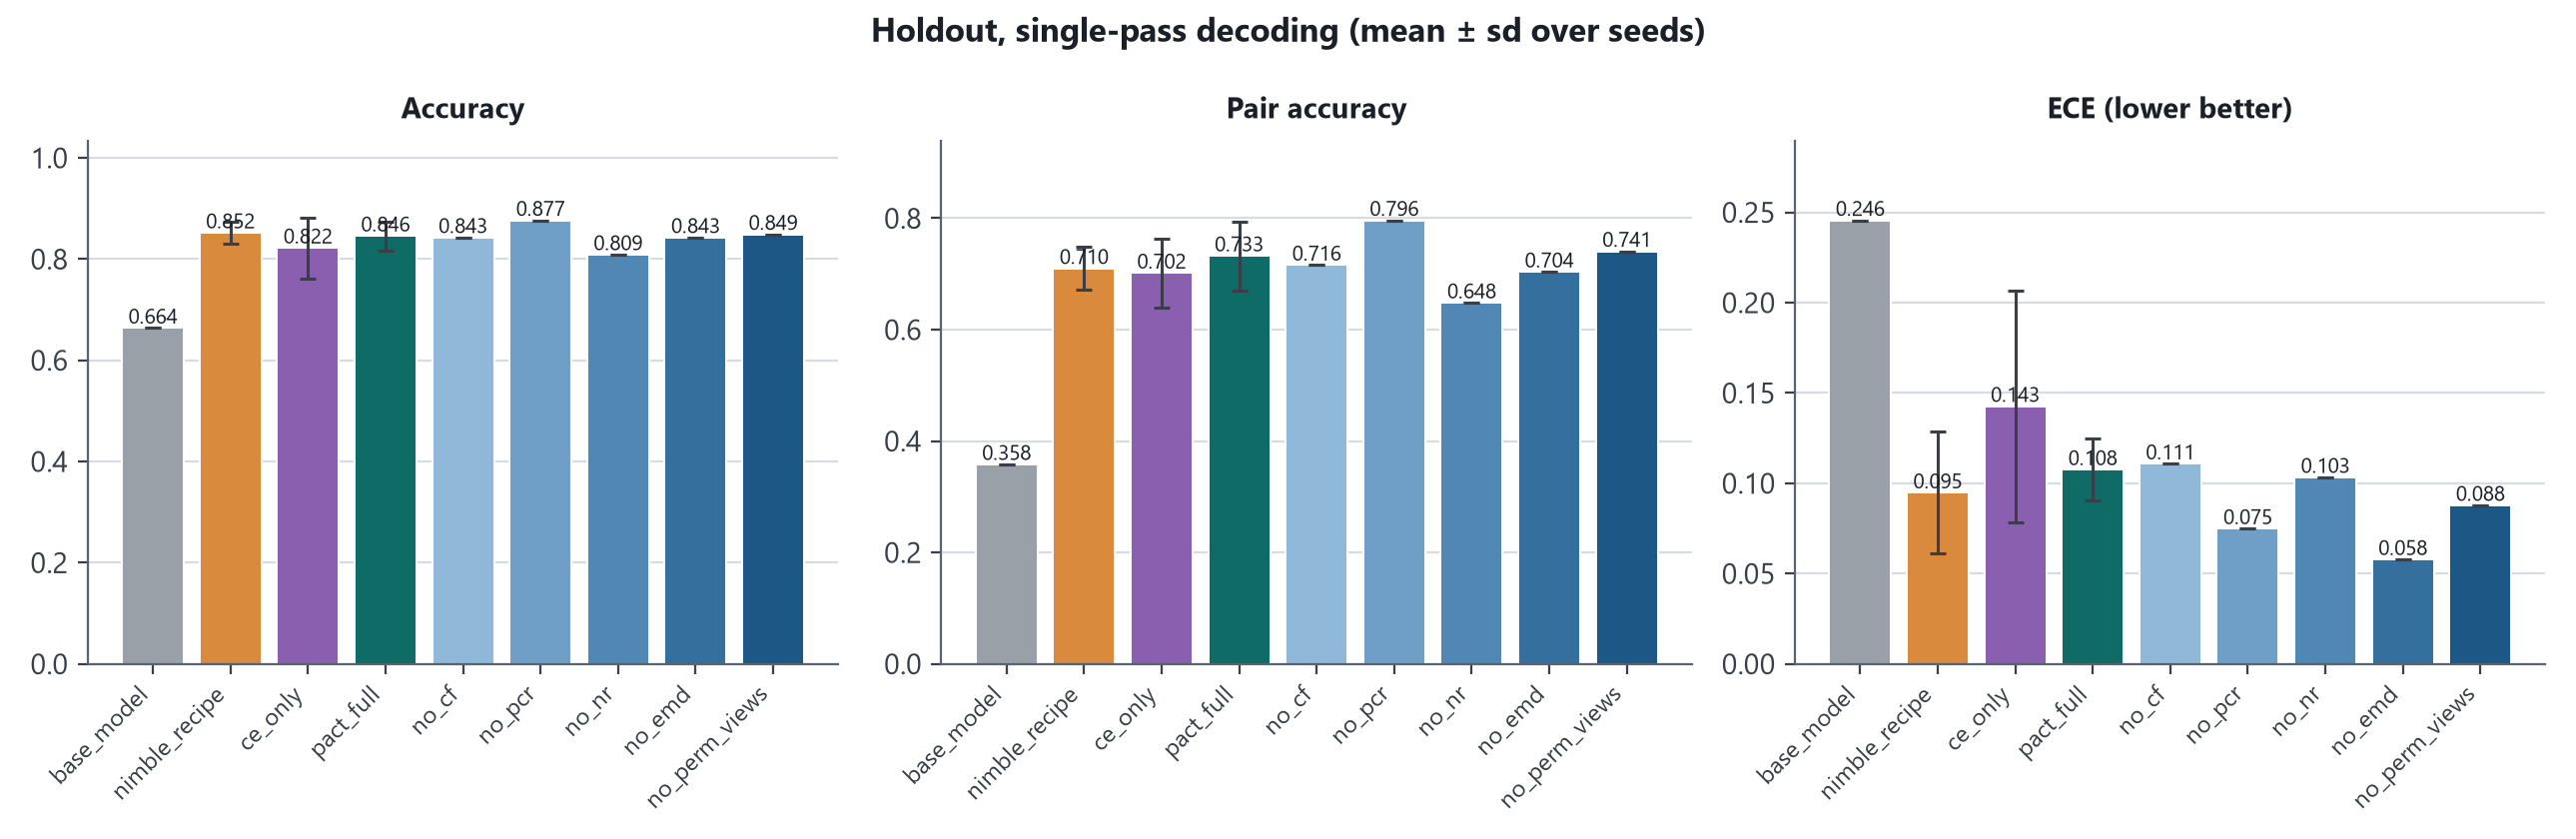
\includegraphics[width=\linewidth]{figures/runs_comparison.png}
\caption{Holdout comparison across runs and ablations, single-pass decoding,
mean $\pm$ standard deviation over seeds. Grey: untouched base model. Amber /
plum: the two reproduced controls. Teal: the full method. Blue ramp: the
five leave-one-out ablations.}
\label{fig:runs}
\end{figure}}{}

\IfFileExists{figures/reliability.png}{%
\begin{figure}[t]
\centering
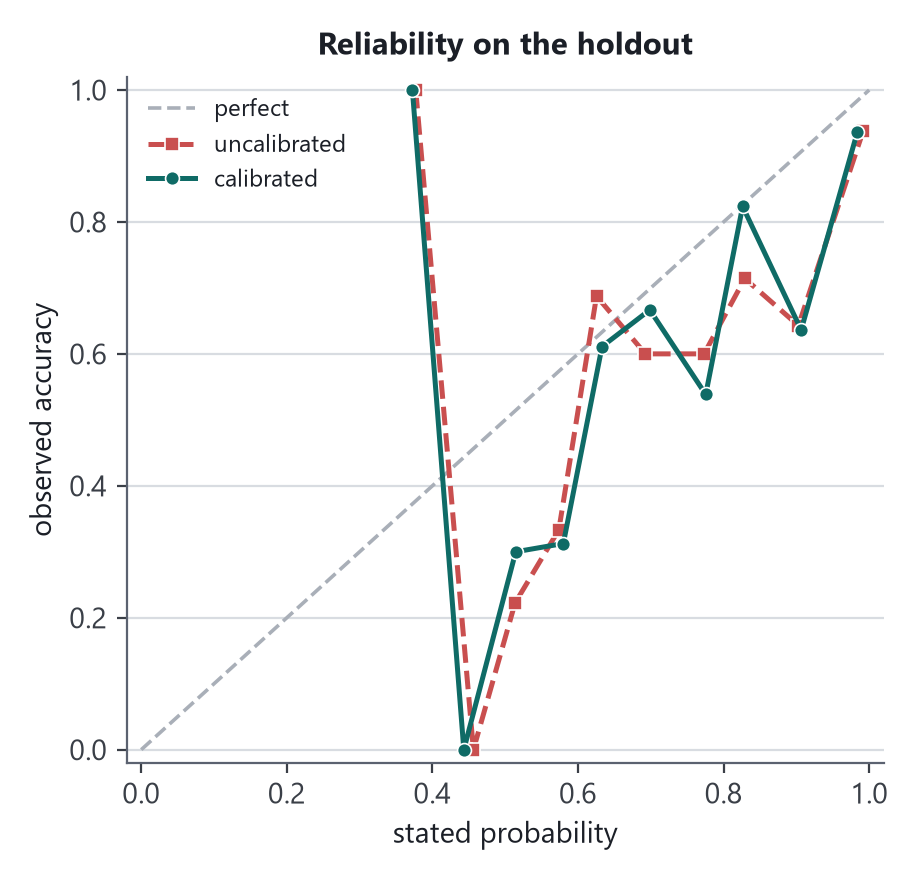
\includegraphics[width=0.48\linewidth]{figures/reliability.png}
\hfill
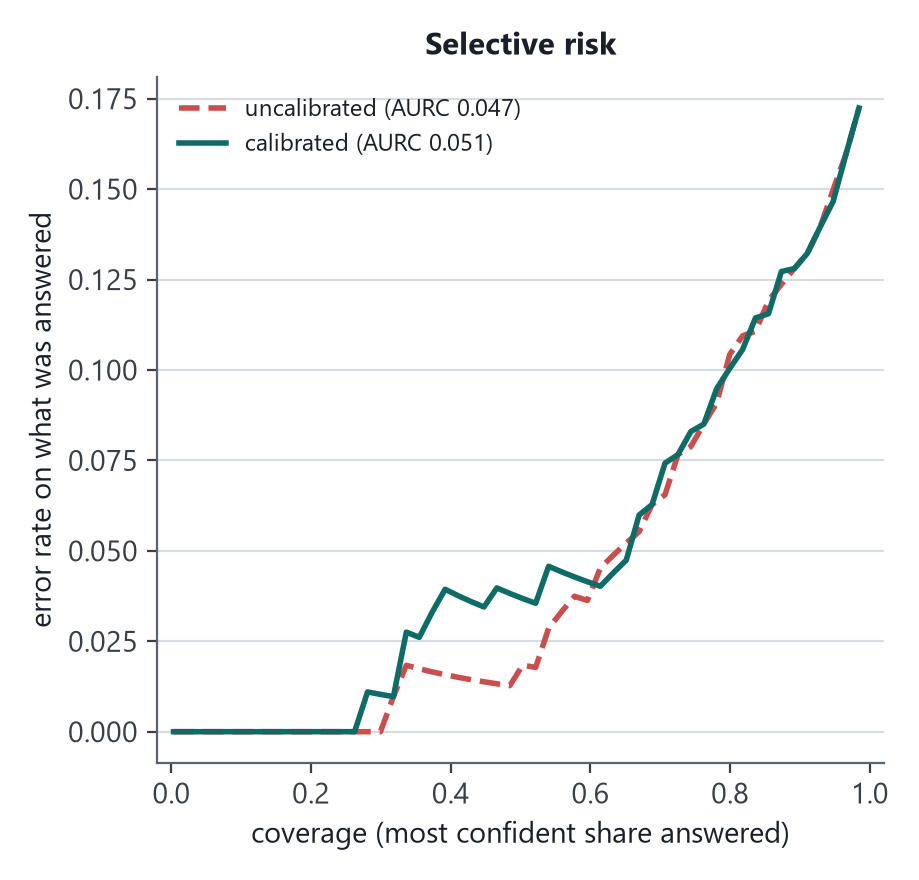
\includegraphics[width=0.48\linewidth]{figures/risk_coverage.png}
\caption{Left: stated probability against observed accuracy on the holdout,
before and after the fitted contextual temperature. Right: error rate
against the share of examples answered, ranked by confidence.}
\label{fig:calibration}
\end{figure}}{}

\IfFileExists{figures/permutation.png}{%
\begin{figure}[t]
\centering
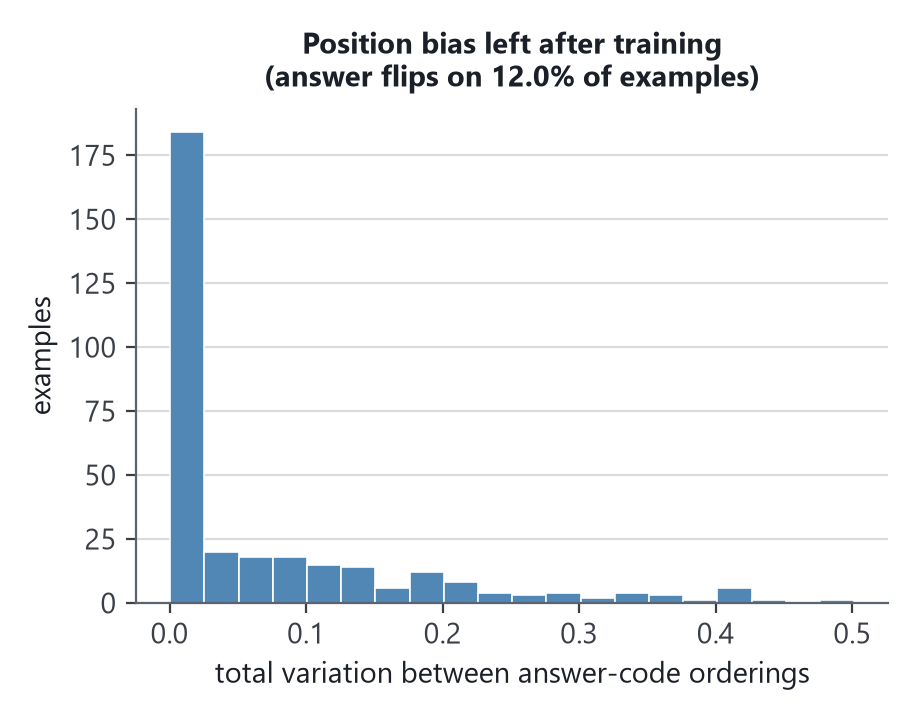
\includegraphics[width=0.6\linewidth]{figures/permutation.png}
\caption{Total-variation distance between the distributions produced
under different answer-code orderings.}
\label{fig:permutation}
\end{figure}}{}

\IfFileExists{figures/ensemble_sweep.png}{%
\begin{figure}[t]
\centering
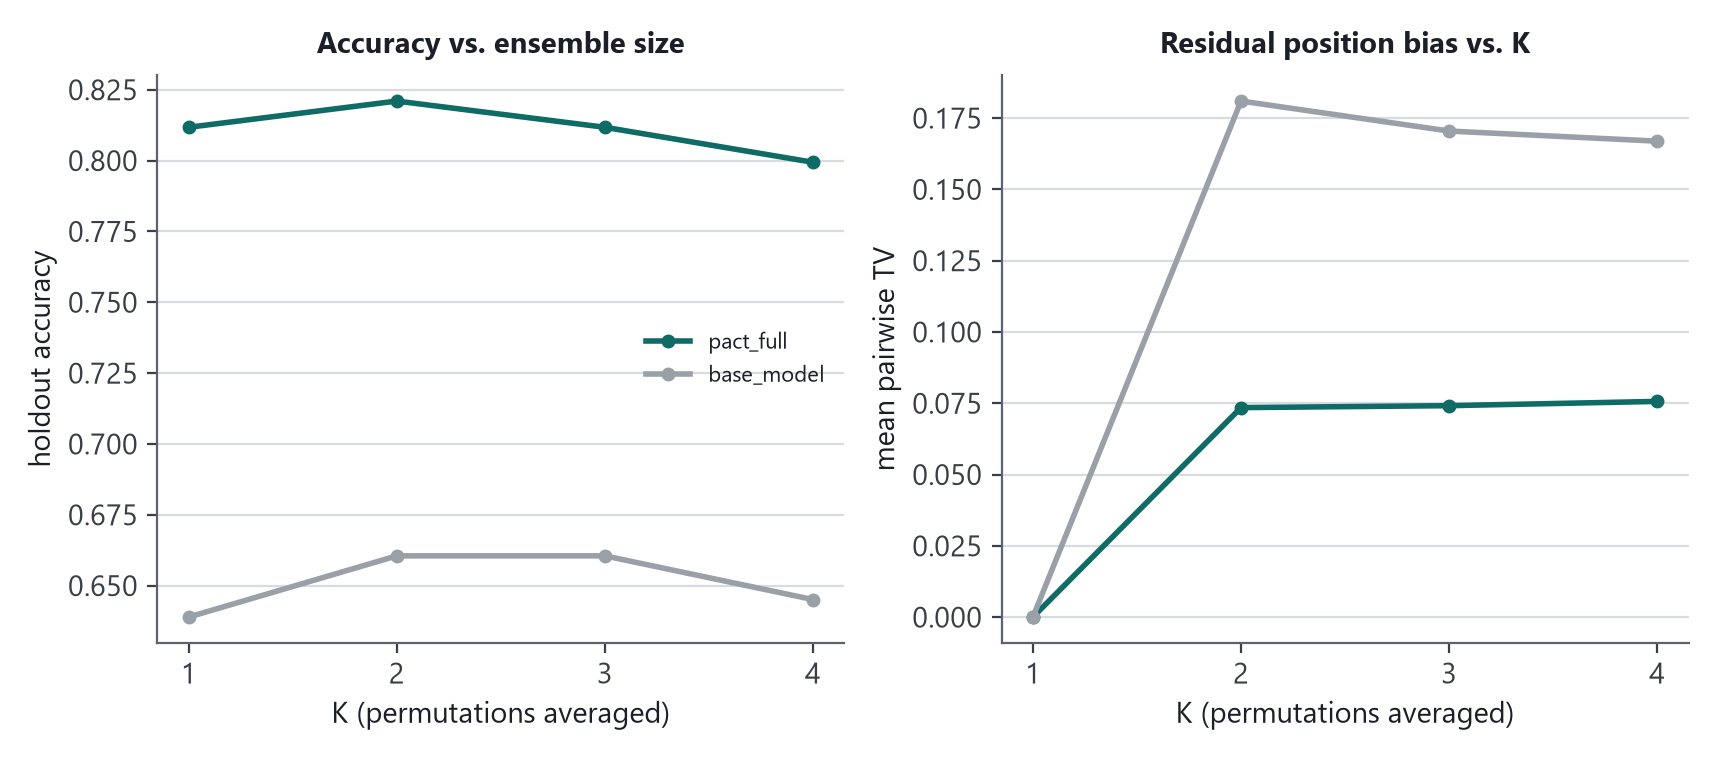
\includegraphics[width=\linewidth]{figures/ensemble_sweep.png}
\caption{Accuracy and residual position bias as the permutation ensemble
size $K$ grows, shipped model vs.\ base model.}
\label{fig:sweep}
\end{figure}}{}

\section{Related work}

\textbf{Serving typed decisions.} Reading candidate-token logits at a single
position, rather than generating and parsing structured text, is the
mechanism behind Jev-style System-One decisions and is described for this
model family by Rogge (2026). Bespoke-MiniCheck (Tang et al., 2024; Bespoke
Labs, 2025) applies the same idea to a single boolean field.

\textbf{Counterfactual and contrastive supervision.} Counterfactually
augmented data (Kaushik et al., 2020) shows that minimal edits that flip a
label reduce reliance on spurious features; contrast sets (Gardner et al.,
2020) use the same construction for evaluation. Both typically feed the
edited examples to an unchanged objective. Our difference-in-differences
margin instead makes the \emph{pairing} part of the loss, and its invariance
to a shared offset is what distinguishes it from simply training on both
members.

\textbf{Position and option-order bias.} Multiple-choice LLM evaluation is
known to depend on option order and label identity (Zheng et al., 2024;
Pezeshkpour and Hruschka, 2024), with debiasing usually applied at inference
by permuting and averaging. We additionally train against it, which is what
makes single-pass serving --- the reason this model family exists --- cheap
again.

\textbf{Calibration.} Temperature scaling (Guo et al., 2017) is the standard
post-hoc method; we keep its objective and let the temperature depend on two
observable prompt statistics.

\textbf{Ordinal targets.} Squared-EMD losses for ordered classes are
standard in label-distribution learning (Hou et al., 2017); we apply them to
rubric fields whose expected level the serving path already computes.

\textbf{Parameter-efficient tuning.} LoRA (Hu et al., 2022) with
rank-stabilised scaling (Kalajdzievski, 2023) and LoRA+ (Hayou et al.,
2024); QLoRA (Dettmers et al., 2023) for the 24\,GB configuration.

\section{Limitations}

The holdout is 324 synthetic, model-labelled examples from six source
families; it is narrow, and its labels were produced by the same family of
models that produced the training labels, so shared errors are possible and
are not detectable from inside the benchmark. $\Lnr$ and $\Lcf$ both trust
the certificate: if a certificate's necessity check is wrong, the necessity
term teaches indifference where the evidence actually decides. We apply the
necessity term to one ablated view per pair, not both, to bound cost.
Permutation ensembling multiplies serving cost by $K$, which is why the
headline comparison uses $K=1$. The five leave-one-out ablations report a
single seed each; \S6.5's significance tests are therefore limited to the
three multi-seed arms, and a claim about any individual loss term's effect
on raw accuracy (as opposed to pair accuracy or calibration, where the
multi-seed arms already carry the evidence) should be read as suggestive, not
confirmed. Finally, all claims here concern one base model at one scale with
one adapter rank.

\section*{References}
{\small
\begin{flushleft}
Bespoke Labs. \emph{Bespoke Nimble: Data, Model, Recipe for an open Jev.} 2026.\\[2pt]
Bespoke Labs, Tang, L., Durrett, G. \emph{Bespoke-MiniCheck.} 2025.\\[2pt]
Dettmers, T., Pagnoni, A., Holtzman, A., Zettlemoyer, L. \emph{QLoRA: Efficient Finetuning of Quantized LLMs.} NeurIPS, 2023.\\[2pt]
Gardner, M., et al. \emph{Evaluating Models' Local Decision Boundaries via Contrast Sets.} Findings of EMNLP, 2020.\\[2pt]
Guo, C., Pleiss, G., Sun, Y., Weinberger, K. \emph{On Calibration of Modern Neural Networks.} ICML, 2017.\\[2pt]
Hayou, S., Ghosh, N., Yu, B. \emph{LoRA+: Efficient Low Rank Adaptation of Large Models.} ICML, 2024.\\[2pt]
Hou, P., Geng, X., Zhang, M.-L. \emph{Squared Earth Mover's Distance-based Loss for Training Deep Neural Networks.} arXiv:1611.05916, 2017.\\[2pt]
Hu, E., et al. \emph{LoRA: Low-Rank Adaptation of Large Language Models.} ICLR, 2022.\\[2pt]
Kalajdzievski, D. \emph{A Rank Stabilization Scaling Factor for Fine-Tuning with LoRA.} arXiv:2312.03732, 2023.\\[2pt]
Kaushik, D., Hovy, E., Lipton, Z. \emph{Learning the Difference that Makes a Difference with Counterfactually-Augmented Data.} ICLR, 2020.\\[2pt]
Pezeshkpour, P., Hruschka, E. \emph{Large Language Models Sensitivity to the Order of Options in Multiple-Choice Questions.} Findings of NAACL, 2024.\\[2pt]
Rogge, N. \emph{Post on single-token decoding for typed decisions}, 2026.\\[2pt]
Tang, L., Laban, P., Durrett, G. \emph{MiniCheck: Efficient Fact-Checking of LLMs on Grounding Documents.} EMNLP, 2024.\\[2pt]
Zheng, C., Zhou, H., Meng, F., Zhou, J., Huang, M. \emph{Large Language Models Are Not Robust Multiple Choice Selectors.} ICLR, 2024.
\end{flushleft}
}

\appendix
\section{Applied demonstration: an interactive decision task}
\label{sec:tetris}

Everything above evaluates the adapter on the task it was trained for: a
static document plus a schema question. As a separate, qualitative check of
how far the same serving mechanism generalises, we reused it unmodified for a
task with no document at all — choosing where to place falling pieces in a
from-scratch Tetris implementation. At every piece, the game engine (not the
model) enumerates every legal placement and works out its consequences two
plies deep — rows cleared, holes created, resulting stack height and skyline
bumpiness, both now and after the best placement of the already-visible next
piece. Each option becomes one \texttt{choice\_description} in an ordinary
\texttt{PactScorer} schema call, exactly the contract \S2.1 describes; the
model reads one token and the highest-logit candidate is played. No part of
the model, the prompt format or the adapter loading path differs from the
main evaluation — only the domain of the schema question changes, from a
business document to a game state.

\paragraph{The shipped adapter, unmodified.} Given this prompting, the
adapter fine-tuned in \S5 does not reliably pick the option the two-ply
search ranks best, even when that option is marked as clearing a line — the
base model this adapter comes from is a general-purpose classifier and was
never trained to weigh sequential-decision trade-offs against each other, and
PACT's training objective (\S3) does not change that; it targets label
accuracy and calibration on the curated pairs, not action selection. This is
the expected outcome, not a failure of \S5's results — it is included here to
be precise about what the held-out accuracy numbers do and do not predict.

\paragraph{Closing the gap with policy-gradient fine-tuning.} We then further
fine-tuned the same LoRA adapter with REINFORCE (single-step, i.e.\ a
contextual bandit over the candidate placements, not full episodic RL),
using the exact two-ply heuristic score of the sampled placement as the
reward and the mean heuristic score across that state's candidates as a
zero-cost, per-state baseline. No architecture, prompt or answer-code changed
— the same \texttt{PactScorer}-compatible PEFT adapter that served \S5's
evaluation is now trained toward a different objective, with training and
serving sharing the identical prompt-construction code so there is no
train/serve skew. The fraction of sampled moves matching the heuristic's own
top-ranked candidate (\texttt{top\_pick\_rate}) rose from 0.19 at step 1 to
$\geq 0.875$ within 200 steps and stayed at 0.75--1.0 for the remainder of
1{,}574 steps on 2$\times$40GB GPUs (full logs and the trained adapter are in
the accompanying repository's \texttt{RL/} bundle). Under a fixed 400-piece
evaluation cap, greedy (argmax) play scored a mean of 17{,}940 at step 50 and
17{,}340 at step 1{,}550 across 5 games each — flat, because the cap is
reached before the model tops out, not because it stopped improving; one
uncapped evaluation game at the final checkpoint reached 1{,}500 pieces,
598 lines and a score of 65{,}700 before we stopped it.

\paragraph{Reading this appendix.} This is a single training run with no
seeds, no held-out repetitions and no statistical test, reported for exactly
what it is: a demonstration that (a) the PACT/Nimble serving contract is a
general typed-choice interface, not something specific to the document
benchmark, and (b) a model shown to be a weak sequential decision-maker
out of the box under that interface can be measurably improved at the
decision task itself, with the same lightweight adapter mechanism, without
touching its document-classification behaviour. It should not be read as
evidence about \S5's holdout claims in either direction.

\end{document}
